\documentclass[12pt,a4paper]{report}
%\documentclass[10pt,a4paper,twocolumn]{report}


%%%%% preamble %%%%%

%%% use package %%%

\usepackage{amsmath,amssymb,amsfonts}
\usepackage{subfigure}
\usepackage{natbib}
\usepackage{setspace}
\usepackage{times}
\usepackage{here}
%\usepackage[dvipdfm]{graphicx}
%\usepackage[dvips]{graphicx}
\usepackage[dvipdfmx]{graphicx}
%\usepackage{color}



%%% text size %%%
\setlength{\topmargin}{20mm}
\addtolength{\topmargin}{-1in}
\setlength{\textheight}{232mm}
\setlength{\headsep}{0mm}
\setlength{\headheight}{0mm}
\setlength{\topskip}{0mm}
\setlength{\oddsidemargin}{30mm}
\addtolength{\oddsidemargin}{-1in}
\setlength{\evensidemargin}{30mm}
\addtolength{\evensidemargin}{-1in}
\setlength{\textwidth}{150mm}
%\setlength{\leftmargin}{-1 in}

\renewcommand{\bibname}{References}

\doublespacing


\sloppy

%%% title information %%%L
\title{
  \Large{Master Thesis}\\[1.5cm]
  \LARGE{\bf Exploring the existence of prebiotic species:\\
    ALMA observations of amine-containing organic molecule in star-forming regions.}\\[3cm]
}
\author{
  \Large{\bf Harumi Minamoto}\\
%  \Large{}\\[0.5cm]
  \large{17M01629}\\
  \large{Nomura Laboratory}\\
  \large{Department of Earth and Planetary Sciences,\,Tokyo Institute of Technology}\\[2cm]
}
\date{\large{\bf \today}}


\input{jnl_list}

%%%%% main page %%%%%
\begin{document}


%%% make title %%%
\maketitle
\thispagestyle{empty}\mbox{}\newpage

\pagenumbering{roman}

%%% abstract %%%
\chapter*{Abstract}
\addcontentsline{toc}{chapter}{Abstract}

\singlespacing
\doublespacing
L
A variety of complex organic moleculues have been observed for decades in the interstellar medium.
Some of them are considered to be delivered to the primordial Earth by comets, 
and contributed to the chemical evolution leading to terrestrial life.
One example of such prebiotic species is amino acid. Glycine, the simplest amino acid, 
has been detected in comet 67P/C-G but its presence in molecular clouds is still uncertain.

In this work we analyze the ALMA archival data toward 3 star-forming regions, 
Orion Kleinmann-Low nebula (hearafter Orion-KL), IRAS 16293-2422 (IRAS 16293), and L483,
to search methylamine (CH$_3$NH$_2$), which is suggested as precursors to glycine. 

As a result of analysis, we found 8 candidate emission at the hot core region in Orion-KL.
By using the rotation diagram method, we evaluated its tentative column density 
and rotational temperature to be 5.5$\times$10$^{14}$ cm$^{-2}$ and 93.3 K, respectively. 
On the other hand, CH$_3$NH$_2$ is not detected and stringent upper limit column densities
are determined in IRAS 16293 and L483.

%%% table of contents %%%
\include{tableofcontents}

%%% main chapters %%%
% Empty pages are inserted to make each title page
% come to the right-hand side (odd page) of the book.
\thispagestyle{empty}\mbox{}\newpage
\chapter{Introduction
  \label{chap:introduction}}

%%% page numbering %%%
\pagenumbering{arabic}

%\section{Origin of life}
%The interstellar medium (ISM), where more than 190 molecules ranging from simple
%linear molecules to complex organic molecules (hereafter COMs) were detected, show
%chemically rich environment. Astronomers usually regard the species with more than six
%atoms as COMs. Not only O-bearing species, CH$_3$OH, CH3OCH3, HCOOCH3, but also
%N-bearing species such as CH3CH2CN and CH2CHCN are known COMs. In 2016, a chiral
%molecule propylene oxide (CH3CHHCH2O) was detected towards Sgr B2 (N) molecular
%cloud in absorption (McGuire et al. 2016). This detection implies that molecules can get
%sufficient complexity, and it will accelerate surveys of other chiral molecules, like amino
%acids.
%From this point of view, many observations were conducted to search for prebiotic
%molecules in the ISM, which might turn into the Seeds of Life when delivered to a
%planetary surface. Especially, a great attention was paid to amino acids, essential building
%blocks of terrestrial life; many surveys were made unsuccessfully to search for the simplest
%amino acid, glycine (NH2CH2COOH), towards Sgr B2 and other high-mass star forming
%regions (e.g., Brown et al. 1979; Snyder et al. 1983; Combes et al. 1996). In 2003, Kuan
%et al. (2003) claimed the %rst detection of glycine, however, several follow-up observations
%concluded denied the detection (e.g., Jones et al. 2007). The difficulty of the past glycine
%surveys would be originated from potential weakness of glycine lines and low sensitivities of
%telescopes used for the surveys.

\section{Glycine and methylamine}
Methylamine is considered as
a precursor of the simplest amino acid glycine. Recent experimental
studies have shown several reaction pathways to forming
glycine in water containing ices starting from CH3NH2 and CO2
subjected to high energy electrons (Holtom et al. 2005) or UV
radiation (Bossa et al. 2009; Lee et al. 2009). Under similar conditions
glycine can decompose to yield methylamine and CO2
(Ehrenfreund et al. 2001). Interstellar methylamine was first detected
toward Sgr B2 at 3.5 cm (Fourikis et al. 1974) and at 3mm
(Kaifu et al. 1974). Recently, methylamine has been detected in
a spiral galaxywith a high redshift of 0.89 located in front of the
quasar PKS 1830-211 (Muller et al. 2011). It was also observed
in cometary samples of the Stardust mission (Glavin et al. 2008).


図(??)にメチルアミンの構造を示す。

\section{Star forming region}
\subsection{Orion Kleinmann-Low nebula}
今回の研究対象としているこのOrion Kleinmann-Low (KL) 天体はオリオン星雲の
中にある赤外線星雲であり、太陽からおよそ437 pc(約1425 光年)離れた位置に存在
している[21]。この領域では、太陽の30 倍の質量をもつ巨大な星が誕生している非常
に活発な領域であり、広い範囲の周波数を観測するline survey でも数多くの分子が観
測されている[5, 22]。このOrion KL は太陽から最も近い位置にある大質量星形成領域
であり、放射強度も強く、なおかつ多くの分子が存在するため、この領域に関しては
1967 年に発見されて以来、line survey を含めた多くの研究が今までにもなされている。
Orion-KL において、多くの有機分子が存在する領域としてHot coreとCompact
ridgeと呼ばれる場所が知られている。Hot core は暖かく($\sim$150 K)、コンパクト(
$<$0.05 pc)で、密度の高い(106 cm-3)領域として知られており[23]、Compact ridge も
同様に暖かく密度の高い領域であることが分かっている[24]。しかし、化学的な性質は
異なっており、Hot core では窒素を含む分子(たとえば、NH3、CH3CN など)が多く
観測される一方で、Compact ridge では酸素を含む分子(たとえば、CH3OH、CH3OCH3
など)が多く発見されている[24]。

\subsection{IRAS 16293-2422}


\subsection{L483}

\section{Radio observation}
電波による宇宙空間の観測は、Karl G. Jansky による1930 年代の初めての宇宙電波
の発見、Grote Reber による世界初の電波望遠鏡の作成以来、宇宙空間の観測方法の1
つとして確立し、また、第2次世界大戦中のレーダー技術の進展を受けて大きな進展を
遂げている。これ以降、X 線や赤外線などの波長でも観測が行われるようになり、可視
光だけではわからない数々の宇宙の不思議を解き明かしている。ただし、大気による吸
収の影響で、全波長のうち地上から観測可能なのは可視光と電波、赤外線の一部となっ
ている。電波の領域では、20 MHz 以下の周波数は電離層を通らず、また高い周波数で
は大気の酸素や水蒸気に吸収されやすい。このため、電波望遠鏡の設置場所としては、
標高が高く、水蒸気が少ない場所が適切である。
可視光や赤外線など観測する波長により、宇宙空間で異なる現象を捉える事ができる
が、電波による宇宙空間の観測では他の波長にはない特徴がある。
・可視光では見えないような低温の物体を観測できる。
生まれた後の星は可視光を放射するが、星が生まれる前の温度の低い天体は可視光を放
射せず、電波を放射している。そのため、このような天体の研究には電波による観測が
必要である。
・波長が長い
この特徴のため、星間微粒子による吸収を受けにくく、奥の方まで観測することができ
る。
・電気的に干渉技術が容易
干渉計と呼ばれる望遠鏡では複数のアンテナを離して置いて観測し、電波を干渉させる
ことにより高い分解能を得ることができるが、電波領域ではこの方法により他の波長に
よる観測よりも高い分解能を得ている。
以上のような特徴により、電波による観測は天文学で重要な位置を占めている。

\subsection{Atacama Large Millimeter Array}
%\subsection{Principle of interferometry}

\section{Purpose of this work}
%\thispagestyle{empty}\mbox{}\newpage
\chapter{Methylamine survey in Orion-KL
\label{chap:Orion-KL}}

\section{Observation data}
%\subsection{Cycle 2}
%\subsection{ALMA Science Verification data}

\section{Analysis}
\subsection{Continuum Subtraction of SV data}
\subsection{Line identification}

\section{Results}
\subsection{Transitions}
\subsection{Distribution}
\subsection{Spectrum}

\section{Disucssion}
\subsection{Column density and Rotation temperature}
\subsection{Blending}
%\thispagestyle{empty}\mbox{}\newpage
\chapter{Methylamine survey in low mass star-forming regions
  \label{chap:LMSFRs}}

\section{Review of low mass star-forming region}
\section{Analysis}

\section{IRAS 16293}
\subsection{Observation data}
\subsection{Results}

\begin{figure}[H]
  \centering
  \includegraphics[width=0.7\textwidth]{LMSFR/IRAS16293_mom0.eps}
  \caption{Integrated intensity map around 247.362 GHz. The white contours represent the 1.3 mm continuum map, where the contour levels are 10 \%, 30 \%, 50 \%, 70 \%, 90 \% of the peak intensity.}
  \label{IRAS16293_mom0}
\end{figure}

\begin{figure}[H]
  \centering
  \includegraphics[width=0.7\textwidth]{LMSFR/IRAS16293.eps}
  \caption{Upper limit column density for the strongest CH$_{3}$NH$_{2}$ transition
  ($7_{2}E_{1-1} \rightarrow 7_{1}E_{1-1}$) as function of T$_{\textrm{rot}}$. A 3$\sigma$ value of 
  11.4 mJy beam$^{-1}$ is used.}
  \label{IRAS16293_MA}
\end{figure}


%\subsubsection{Transitions}
%\subsubsection{Integrated intensity map}
%\subsubsection{Upper limit column density}

\section{L483}
\subsection{Observation data}
\subsection{Results}

\begin{figure}[H]
  \centering
  \includegraphics[width=0.7\textwidth]{LMSFR/L483_mom0.eps}
  \caption{Integrated intensity map around 217.079 GHz. The white contours represent the 1.3 mm continuum map, where the contour levels are 10 \%, 30 \%, 50 \%, 70 \%, 90 \% of the peak intensity.}
  \label{L483_mom0}
\end{figure}

\begin{figure}[H]
  \centering
  \includegraphics[width=0.7\textwidth]{LMSFR/L483.eps}
  \caption{Upper limit column density for the strongest CH$_{3}$NH$_{2}$ transition
  ($11_{2}A_{1} \rightarrow 11_{2}A_{2}$) as function of T$_{\textrm{rot}}$. A 3$\sigma$ value of 
  22.5 mJy beam$^{-1}$ is used.}
  \label{L483_MA}
\end{figure}


%\subsubsection{Transitions}
%\subsubsection{Integrated intensity map}
%\subsubsection{Upper limit column density}
%\thispagestyle{empty}\mbox{}\newpage
\chapter{Discussion
  \label{chap:discussion}}

\section{Column density and Rotation temperature}

In this subsection we will describe the methodologies in deriving the column density and the rotational temperature of COMs.
The column density of CH$_{3}$NH$_{2}$ ($N_{\mathrm{MA}}$) was estimated by using 
the rotational temperature diagram method, which assumes local thermodynamic equilibrium 
(LTE) and optically thin emission. 
The following equation was employed for the analysis \citep{Turner1991}:
\begin{align}
\log \dfrac{3\,k_{\mathrm{B}}\,T_{\mathrm{B}} \,\Delta V_{1/2}}{8\, \pi^3\, \nu\, S\, \mu_0^2} = \log \dfrac{N_{\mathrm{MA}}}{U_{\mathrm{rot}}} - \dfrac{E_{\mathrm{u}}}{k_{\mathrm{B}}} \dfrac{\log e}{T_{\mathrm{rot}}}
\label{eq:RD}
\end{align}

In the expression, $\nu$ is the rest frequency of the transition, $\mu_0$ is the permanent dipole moment, 
$U_{\mathrm{rot}}$ is the rotational partition function, $S$ is the line strength, 
$E_{\mathrm{u}}$ is the upper state energy, and $ T_{\mathrm{B}}$ and  $\Delta V_{1/2}$ 
are the brightness temperature and line widths (FWHM, in~km~s$^{-1}$), respectively.
We assumed the average $\Delta V_{1/2} = 4.2\, \mathrm{km\,s^{-1}}$, which derived by the Gaussian fitting.

The brightness temperature can be converted from intensity $I_{\mathrm{\nu}}$
when the Rayleigh-Jeans law is applicable.
\begin{align}
T_{\mathrm{B}} = \dfrac{c^2}{2\,k_{\mathrm{B}}\, \nu^2} \,I_{\mathrm{\nu}}
\end{align}

\begin{figure}[H]
  \centering
  \includegraphics[width=0.8\textwidth]{OrionKL/RD_6point_label.eps}
  \caption{Rotation diagram of CH$_{3}$NH$_{2}$ in Hot core. The error bars represents $\pm$ 3 $\sigma$ for each data.}
  \label{fig:RD}
\end{figure}

The resulting plots are given in Figure \ref{fig:RD}.
The analysis yields a rotational temperature of $T_{\mathrm{rot}} =  95.4^{+15.5}_{-11.7} \,\,\mathrm{K}$, 
with a column density of $N_{\mathrm{MA}} = ( 5.5^{+1.6}_{-1.1} ) \times 10^{14} \,\,\mathrm{cm^{-2}}$.

\section{Suspicious lines}
Comparison of catalogs did not suggest contamination, but some emission lines could not be detected as CH$_{3}$NH$_{2}$.

\renewcommand{\arraystretch}{1.5}
\begin{table}[htb]
\begin{center}

  \caption{transitions of CH$_3$NH$_2$}
  \label{tab:unresolved}
{\scriptsize
  \begin{tabular}{cccccccl} \hline
   Fequency [GHz]& S$\mu ^{2}$ [D$^2$] & E$_{\rm{u}}$ [K]& Transition ($J$, $K_{\rm{a}}$, $\Gamma$) 
   & peak $T_{\mathrm{B}}$\footnotemark[1] [K] & $V_{\mathrm{LSR}}$\footnotemark[1] [km s$^{-1}$] & Noise [K]  &Comments \\ \hline 
    215.670 & 53.92 & 111.48 & 9, 2, $E_{1-1}$ $\rightarrow$ 9, 1, $E_{1+1}$  & 3.74(0.07) & 5.37(0.07) & 0.043 &  \\
    221.755 & 35.06 & 133.11 & 10, 2, $A_{2}$ $\rightarrow$ 10, 1, $A_{1}$ & 0.33(0.03)& 5.35(0.19) & 0.133 &SV data \\ \hline
  \end{tabular}
  }
\end{center}
\end{table}
\footnotetext[1]{Numbers in parenthesis represent standard deviation in the unit of the last significant digits.}


As shown in Figure \ref{fig:RD_blend}, the CH$_{3}$NH$_{2}$ data including 2 transitions in Table \ref{tab:unresolved} 
produced point-to-point scatter perhaps because of the lower signal-to-noise ratio for the weaker transitions in SV data 
and possible high-level contamination.

\begin{figure}[htp]
  \centering
  \includegraphics[width=0.7\textwidth]{OrionKL/RD_blend.eps}
  \caption{Rotation diagram of CH$_{3}$NH$_{2}$ in Hot core with additional 2 lines. The error bars on round plots represents $\pm$ 3$\sigma$ for each data. A signal below 3$\sigma$ is represented by a triangle with the error bar indicating the upper limit. The blue line is the same one as Figure \ref{fig:RD}.}
  \label{fig:RD_blend}
\end{figure}

\subsection*{215.670 GHz line}
This emission line ($E_{\mathrm{u}}=111$ K) is seen at Hot core and IRc7 like other CH$_{3}$NH$_{2}$ transitions 
(see Figure 4.3 and Figure \ref{ch_4}), but this line has stronger intensity than that predicted in the rotation diagram (see Figure \ref{fig:RD_blend}).
Since the line width is also wider than the other CH$_{3}$NH$_{2}$ transitions (see Figure 4.3), 
it appears that this line is blended with other molecular emission lines existing in Hot core.
Then examining the catalog including the transition of higher excitation, CH$_3$CH$_2$CN (215.6687 GHz, $E_{\mathrm{l}}$ = 604.845 K)
has come up as a candidate for blending.
However, considering that T$_{\mathrm{rot}}$ of CH$_3$CH$_2$CN in Hot core is 155 K \citep{Feng+2015}, 
it is uncertain how much this transition of higher excitation contributes to the blending.

\begin{figure}[htp] 
\begin{center}
\begin{minipage}{0.98\textwidth} 
\begin{center}
\begin{minipage}{0.48\textwidth}
\begin{center}
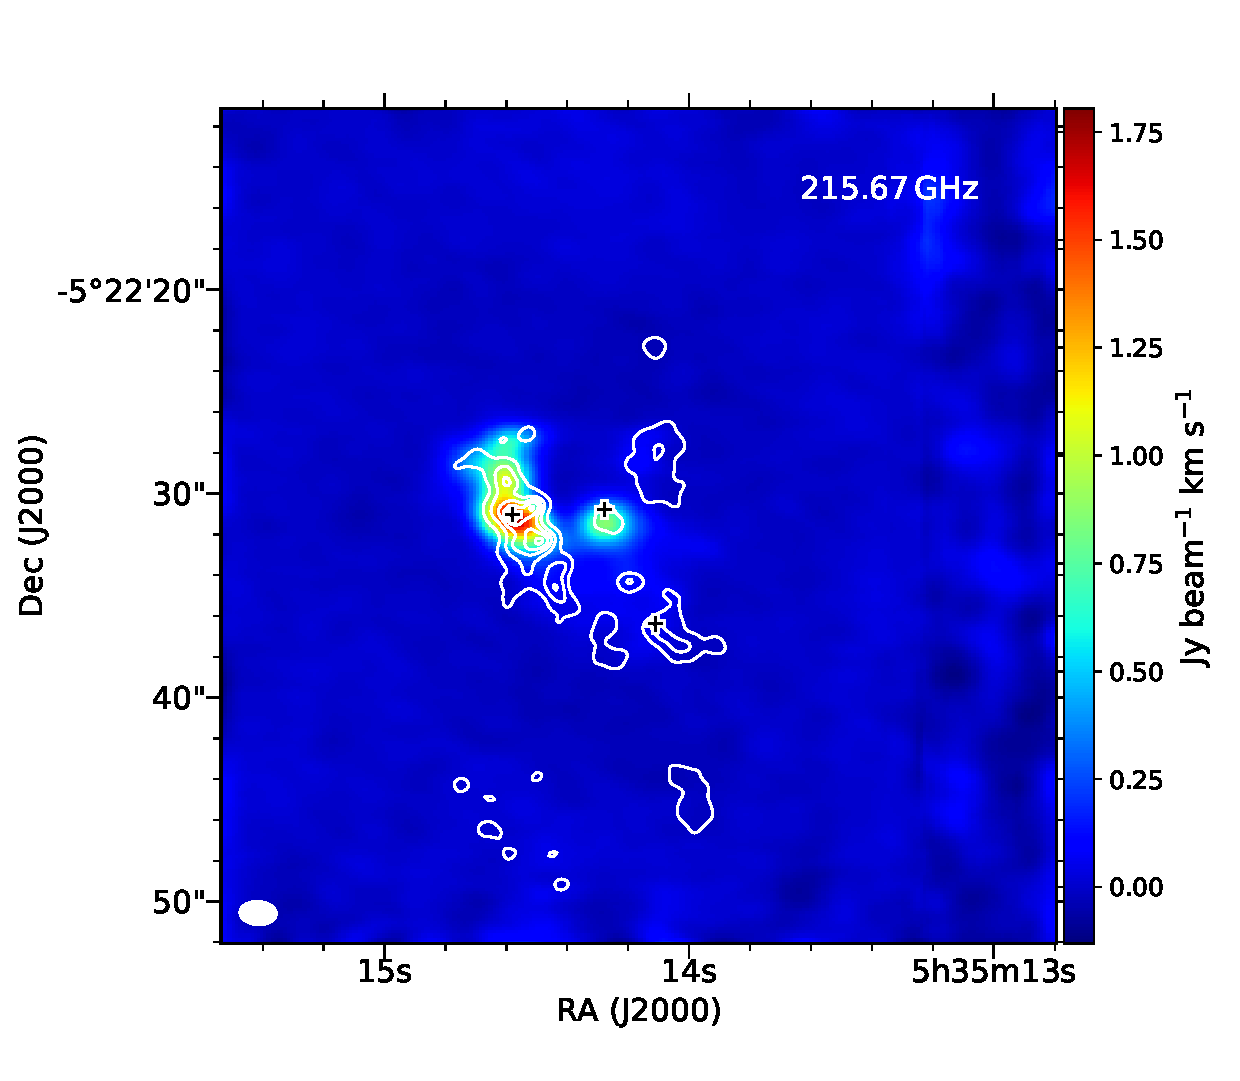
\includegraphics[width=0.98\textwidth]{OrionKL/mom0/215.67mom0_3-7.eps}
\end{center}
\end{minipage}
\begin{minipage}{0.48\textwidth}
\begin{center}
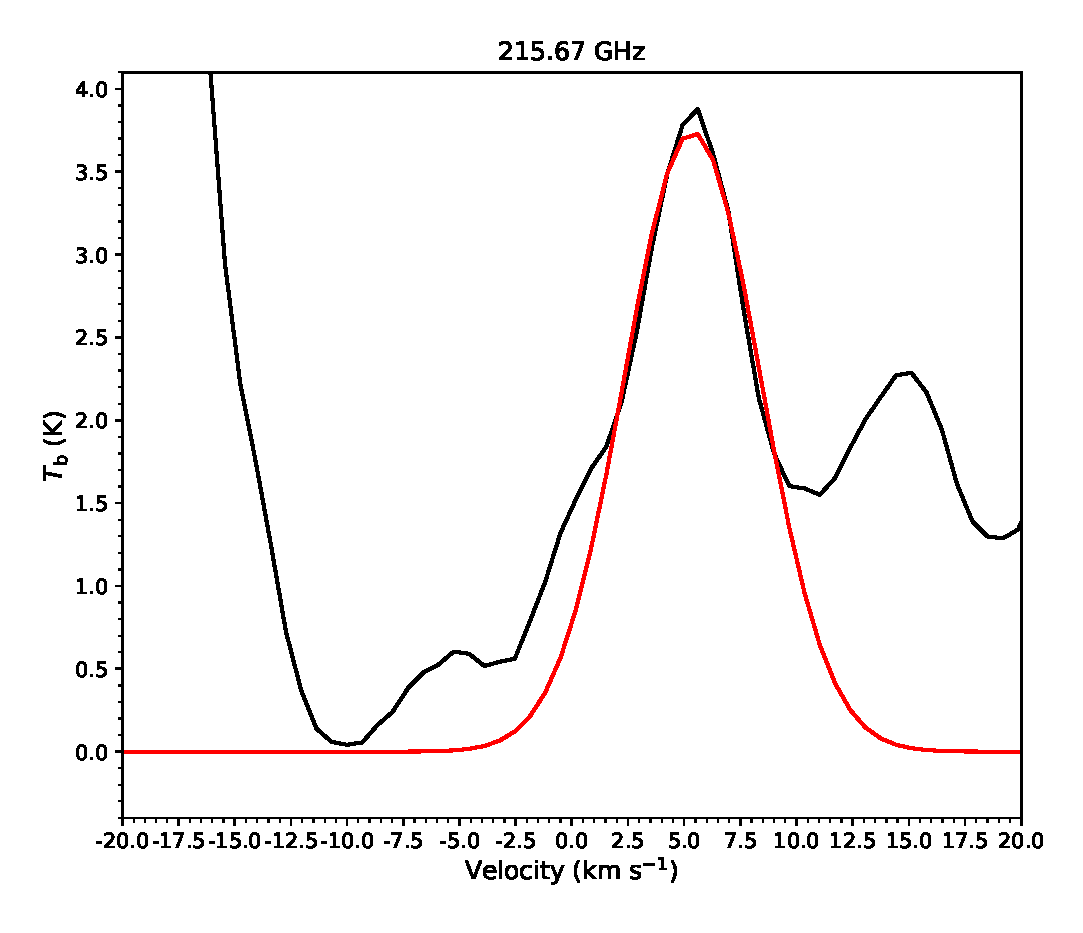
\includegraphics[width=0.98\textwidth]{OrionKL/spectrum/HC/215.6696452w_fit.eps}
\label{fig:215spec}
\end{center}
\end{minipage}
\end{center}
\end{minipage}
\label{fig:215data}
\caption{(left) Integrated intensity map of the emission for 215.670 GHz. Same as Figure \ref{fig:mom0s} but for white contours and black crosses. (right) Spectrum of the CH$_3$NH$_2$ lines at each frequency observed in Hot core (black)  and the result of the Gaussian fitting assuming the average $\Delta V_{1/2} = 4.2\, \mathrm{km\,s^{-1}}$ (red)}
\end{center}
\label{fig:215data}
\end{figure}

\subsection*{221.755 GHz line}
A faint signal was seen in Hot core in the integrated intensity map and channel maps (Figure 4.4 and \ref{ch_6}).
Since there was no blend of other molecular emission lines in the comparison with the catalogs, we analyzed the spectrum, 
but the peak intensity ( $T_{\mathrm{B}}=$ 0.33 K) was weaker than 
3 $\sigma $ noise level ($T_{\mathrm{B}}=$ 0.133 K, see Table \ref{tab:unresolved}). 
When we plotted this line on the rotation diagram with 3$\sigma$ as the upper limit of the intensity, 
the derived value was consistent with other CH$_3$NH$_2$ transitions (see Figure \ref{fig:RD_blend}). 
This emission line was included in SV data cube, 
so it could be possible to detect the line in future observations with higher S/N ratio.

\begin{figure}[htp] 
\begin{center}
\begin{minipage}{0.98\textwidth} 
\begin{center}
\begin{minipage}{0.48\textwidth}
\begin{center}
\includegraphics[width=0.98\textwidth]{OrionKL/mom0/221.755SV_mom0_3-7.eps}
\label{fig:221mom}
\end{center}
\end{minipage}
\begin{minipage}{0.48\textwidth}
\begin{center}
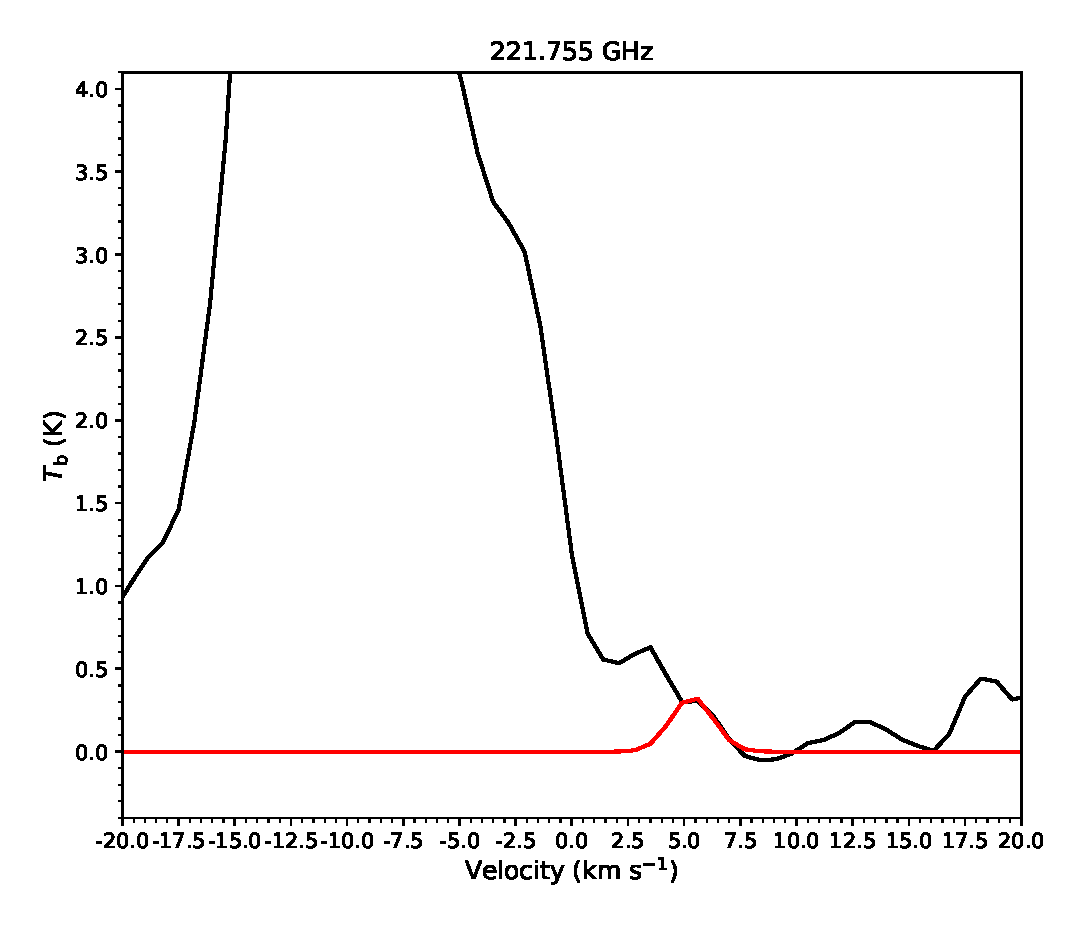
\includegraphics[width=0.98\textwidth]{OrionKL/spectrum/HC/221.755055w_fit.eps}
\end{center}
\end{minipage}
\end{center}
\end{minipage}
\caption{(left) Integrated intensity map of the emission for 221.755 GHz. Same as Figure \ref{fig:mom0s} but for white contours and black crosses. (right) Spectrum of the CH$_3$NH$_2$ lines at each frequency observed in Hot core (black)  and the result of the Gaussian fitting assuming the average $\Delta V_{1/2} = 4.2\, \mathrm{km\,s^{-1}}$ (red)}
\end{center}
\end{figure}

\begin{figure}[htp]
  \centering
  \includegraphics[width=0.98\textwidth]{OrionKL/chmap/215.67.eps}
  \caption{Channel map around 215.670 GHz. Same as Figure \ref{ch_0} but for white contours and mazenta crosses.}
  \label{ch_4}
\end{figure}

\begin{figure}[htp]
  \centering
  \includegraphics[width=0.98\textwidth]{OrionKL/chmap/221.755.eps}
  \caption{Channel map around 221.755 GHz line. Same as Figure \ref{ch_0} but for white contours and mazenta crosses.}
  \label{ch_6}
\end{figure}

%\thispagestyle{empty}\mbox{}\newpage
\chapter{Conclusions
  \label{chap:conclusions}}

In order to ascertain whether the presence of CH$_3$NH$_2$, a precursor of glycine, in the star-formation regions is universal  
 and further to accelerate the discussion regarding the exogenous delivery of 
prebiotic species to planets and connection between the Universe and life,
we explored the existence of CH$_3$NH$_2$ in 3 star-forming regions using ALMA archival data.

As a result of the analysis, CH$_3$NH$_2$ was not detected in low mass star-forming regions 
(see Appendix A), but some emission lines was detected in Orion-KL.

According to the analysis, the physical properties of CH$_3$NH$_2$ were found as follows.
\begin{itemize}
\item From the integrated intensity maps, CH$_3$NH$_2$ concentrates in Hot Core.
\item $V_{\mathrm{LSR}}$ and FWHM line width are estimated to be 4.84~$\pm$~0.22~km~s$^{-1}$ 
and 4.16~$\pm$~0.22~km~s$^{-1}$, respectively. $V_{\mathrm{LSR}}$ are consistent with 
those of N-bearing COMs observed toward Hot core.
On the other hand, $\Delta V_{1/2}$ of CH$_3$NH$_2$ is narrower than those of other molecule in Hot core.
\item By using the rotation diagram method, we evaluated its $T_{\mathrm{rot}}$ and $N_{\mathrm{MA}}$ to be $95.4^{+15.5}_{-11.7} \,\,\mathrm{K}$, and $ (\,5.5^{+1.6}_{-1.1}\,) \times 10^{14} \,\,\mathrm{cm^{-2}}$,  respectively.
\end{itemize}

The distribution and spectrum parameters ($V_{\mathrm{LSR}}$ and FWHM line width) of CH$_3$NH$_2$ in Orion-KL is reported for the first time.
Regarding its rotational temperature and column density, we gave more restrictions than previous studies.

However, since contamination is not sufficiently studied, this detection is still tentative.
We need further line identification including other frequency bands to constrain $T_{\mathrm{rot}}$ and $N_{\mathrm{MA}}$.




%\thispagestyle{empty}\mbox{}\newpage

%%% appendix %%%
\appendix
\include{app_appendix}
%\thispagestyle{empty}\mbox{}\newpage

%%% acknowledgment %%%
\chapter*{Acknowledgments}
\addcontentsline{toc}{chapter}{Acknowledgments}

This work would have been never completed if anyone of greatest persons and colleagues mentioned below is missing.

I would like to express my gratitude my supervisor, Associate Professor Hideko Nomura, for her great
directions, fruitful discussions, and persistent encouragement.
I would like to do the same to Dr. Tomoya Hirota and Dr. Masatoshi Oh'ishi, who led me to the field of radio astronomy.
As for the data analysis of the ALMA telescope, Dr. Yoko Oya, Dr. Toshiki Saito, and Dr. Ryohei Kawabe gave me elaborate guidance.
I also received generous warm support and comments from Dr. Taiki Suzuki, Seongjoong Kim, and Wei Chen-en.

Finally, I am grateful to all of the colleagues of planetary groups at Tokyo Tech, and the seminar mates of ALMA interferometer seminar at National Astronomical Observatory of Japan (NAOJ) for scientific discussion and enjoyable life.


%\thispagestyle{empty}\mbox{}\newpage


%% 本編終了

%% referenceの表示

\addcontentsline{toc}{chapter}{References}

\bibliographystyle{apj}
\bibliography{references}%{references.bib}


\end{document}
